\setstretch{1.4}
\sectiontitle{4}{Software Refactoring}
\lhead{Software Refactoring} % section header
As mentioned in the introduction, this thesis builds upon the work and code developed for a previous iteration of the system. However, the control code, implemented in C++ using Qt, lacked the structure and readability to allow the expansions necessary for this thesis. There was clear room for improvement, especially when it came to modularization, exemplified by the MainWindow class that managed several distinct functionalities and over 80 different member variables. Therefore, before continuing on with the project, a full refactoring of the code was necessary. The objective was to save time in the long run by creating modular, robust, readable code that could easily be further built upon and used in future projects.

\lhead{Software Refactoring - Theory} % section header
\subsection{Theory}
\subsubsection{Software architecture for real-time systems}
Real-time systems require software that is predictable and responsive, even under strict timing constraints. This places additional demands on the software design, especially since codebases for such systems may grow rapidly when there is a necessity for GUI handling, hardware commands, control calculations, and communication protocols. According to McConnel \cite{steve_mcconnell_code_nodate}, high-quality architecture in such systems should emphasize simplicity, clarity, and robustness to change. 

A well-structured architecture improves maintainability and extensibility by making the system easier to understand and reason about. In real-time contexts, this often translates into an architecture that minimizes dependencies between components and provides clear separation between hardware interaction, control logic, and application-level coordination \cite{tanenbaum_distributed_2007}.

\subsubsection{Modular design principles}
Modularity is one of the most important design principles when managing software complexity. Modular systems break down functionality into discrete units that encapsulate behavior and expose minimal interfaces \cite{steve_mcconnell_code_nodate}. This separation reduces the mental burden on developers and allows individual parts of the system to be developed, tested, and modified independently, greatly improving maintainability and scalability.

Effective modularity hinges on two key design goals: low coupling and high cohesion. Low coupling refers to modules having minimal dependencies on each other, and high cohesion means that all parts of a module contribute to a single, clear purpose \cite{steve_mcconnell_code_nodate}. These ideas build on the concept of "information hiding" \cite{parnas_criteria_1972} where internal implementation details are kept private, preventing unintended interactions across modules.

\subsubsection{Threading and concurrency}
Concurrency is often necessary in real-time systems to meet timing constraints and maintain responsiveness. Use of threads allows the system to perform multiple tasks concurrently, such as sensor data acquisition, visualization, control loop computation and user interaction, without blocking the main execution path.

However, introducing concurrency also introduces complexity. Issues such as race conditions, deadlocks and nondeterministic behavior must be managed. McConnell \cite{mcconnell_code_2004} warns that improperly designed concurrency can reduce the reliability of software rather than improve performance. Therefore, concurrent systems should be built using a clear design, thread-safe communication mechanisms and minimal shared states \cite{noauthor_software_nodate}.

\subsubsection{Event-driven communication in Qt}
A common and reliable pattern for concurrent real-time systems is event-driven communication between threads. In this model, components communicate through asynchronous messages rather than direct calls or shared variables. In Qt this is implemented via the signal-slot mechanism. Signals are emitted when events occur, and slots (connected handler functions) respond to those events. Qt ensures that the communication is thread safe by serializing signal delivery using the event loop of the receiving thread, meaning that it will execute in the context of the receiving threads event loop. 

\lhead{Software Refactoring - Methods} % section header
\subsection{Methods}
\subsubsection{Analysis of the original code base}
The refactoring process began with an analysis of the existing codebase. The existing methods and classes were documented and their interactions were visualized in figure such as \ref{fig:oldarchitecture}. This provided an overview of the software architecture and highlighted areas where the structure violated modular design principles, such as excessive coupling and low cohesion. 
\begin{figure} [H]
    \centering
    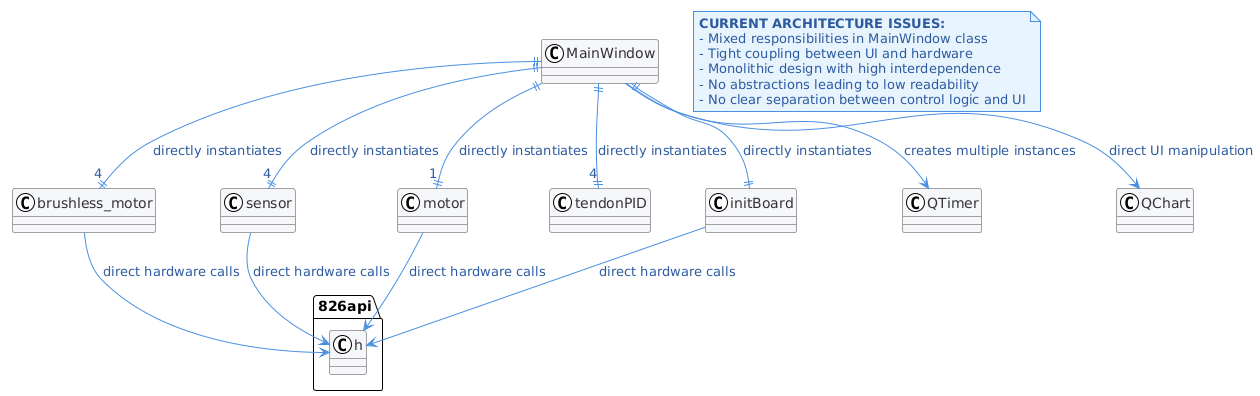
\includegraphics[width=1.1\linewidth]{images/Software documentation/old code/architecture2.png}
    \caption{Original architecture, prior to refactoring}
    \label{fig:oldarchitecture}
\end{figure}

An analysis of the original codebase revealed that the main issue was the low cohesion and large amount of responsibilities and data managed by the \texttt{MainWindow} class, as is exemplified in figure \ref{fig:oldmainwindow}. It also showed that even though the original architecture seen in \ref{fig:oldarchitecture} looks seemingly modularized into relevant modules such as \texttt{motor} and \texttt{tendonPID}, those classes did not have ownership of the appropriate methods or data. The elements that should have been implemented in those classes largely remained in the \texttt{MainWindow} class. This resulted in high interdependence, with little abstraction and low readability.
 \begin{wrapfigure}[25]{r}{0.45\textwidth}
    \centering
    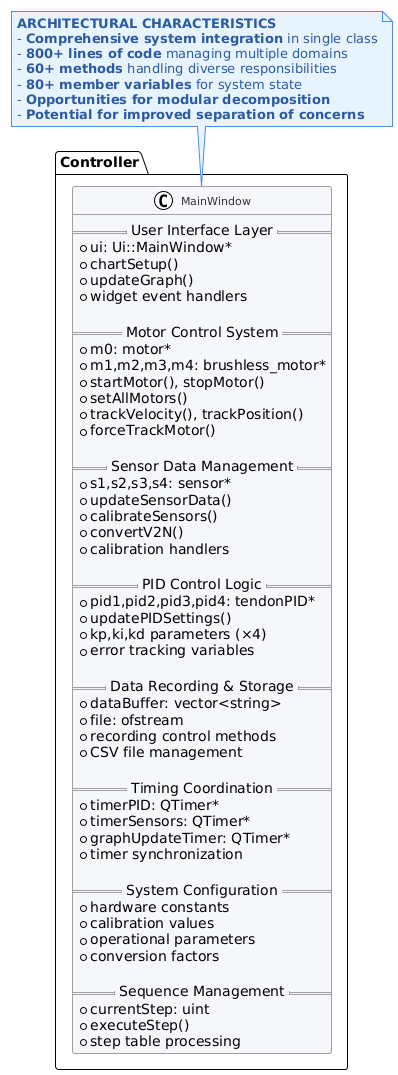
\includegraphics[width=\linewidth]{images/Software documentation/old code/mainwindow2.png}
    \caption{\texttt{MainWindow} implementation, prior to refactoring}
    \label{fig:oldmainwindow}
\end{wrapfigure}

\subsubsection{Restructuring Methodology}
Based on the architectural guidelines described in the theory section, a revised design was developed. The design emphasizes smaller highly cohesive classes and separation of concerns by defining minimal, well-documented interfaces between modules and isolating hardware-dependent functionality, for different types of application level logic. The existing code was refactored to fit into this structure and unnecessary functionality was removed. Existing errors in the code were also remedied. Thereafter new code was written into the modules in order to expand the functionality of the system.

\lhead{Software Refactoring - Results} % section header
\subsection{Results}

\subsubsection{Modularization}
The code was restructured into well defined classes, each responsible for a specific task. These classes were further grouped into folders, these folders are very briefly described in the table below. A description of all the classes can also be found in the appendix. 

\begin{table}[htbp]
\centering
\caption{High Level Descriptions of Software Folder Organization}
\begin{tabular}{p{0.3\textwidth}p{0.65\textwidth}}
\toprule
\textbf{Module} & \textbf{Description} \\
\midrule
Root Directory & Main application framework includes \texttt{MainWindow}, \texttt{Logger}, \texttt{sensor}, and classes responsible for running specific sequences such as \texttt{Tester} and \texttt{AirCalibrator}. \\
\addlinespace
Motor Control & Hardware control modules for linear stage positioning and brushless motor actuation with motion estimation. \\
\addlinespace
Tendon PID Control & Closed-loop tension control system managing individual tendon forces through coordinated PID controllers. \\
\addlinespace
Vision System & Communication interface with Python-based vision system for real-time tip tracking and recording control via ZeroMQ messaging. \\
\addlinespace
Path Following & Trajectory planning and guidance algorithms including line-of-sight navigation, feedback control, and curvature-to-tension mapping. \\
\bottomrule
\end{tabular}
\end{table}


\subsubsection{Architecture}
\begin{figure} [H]
	\centering
	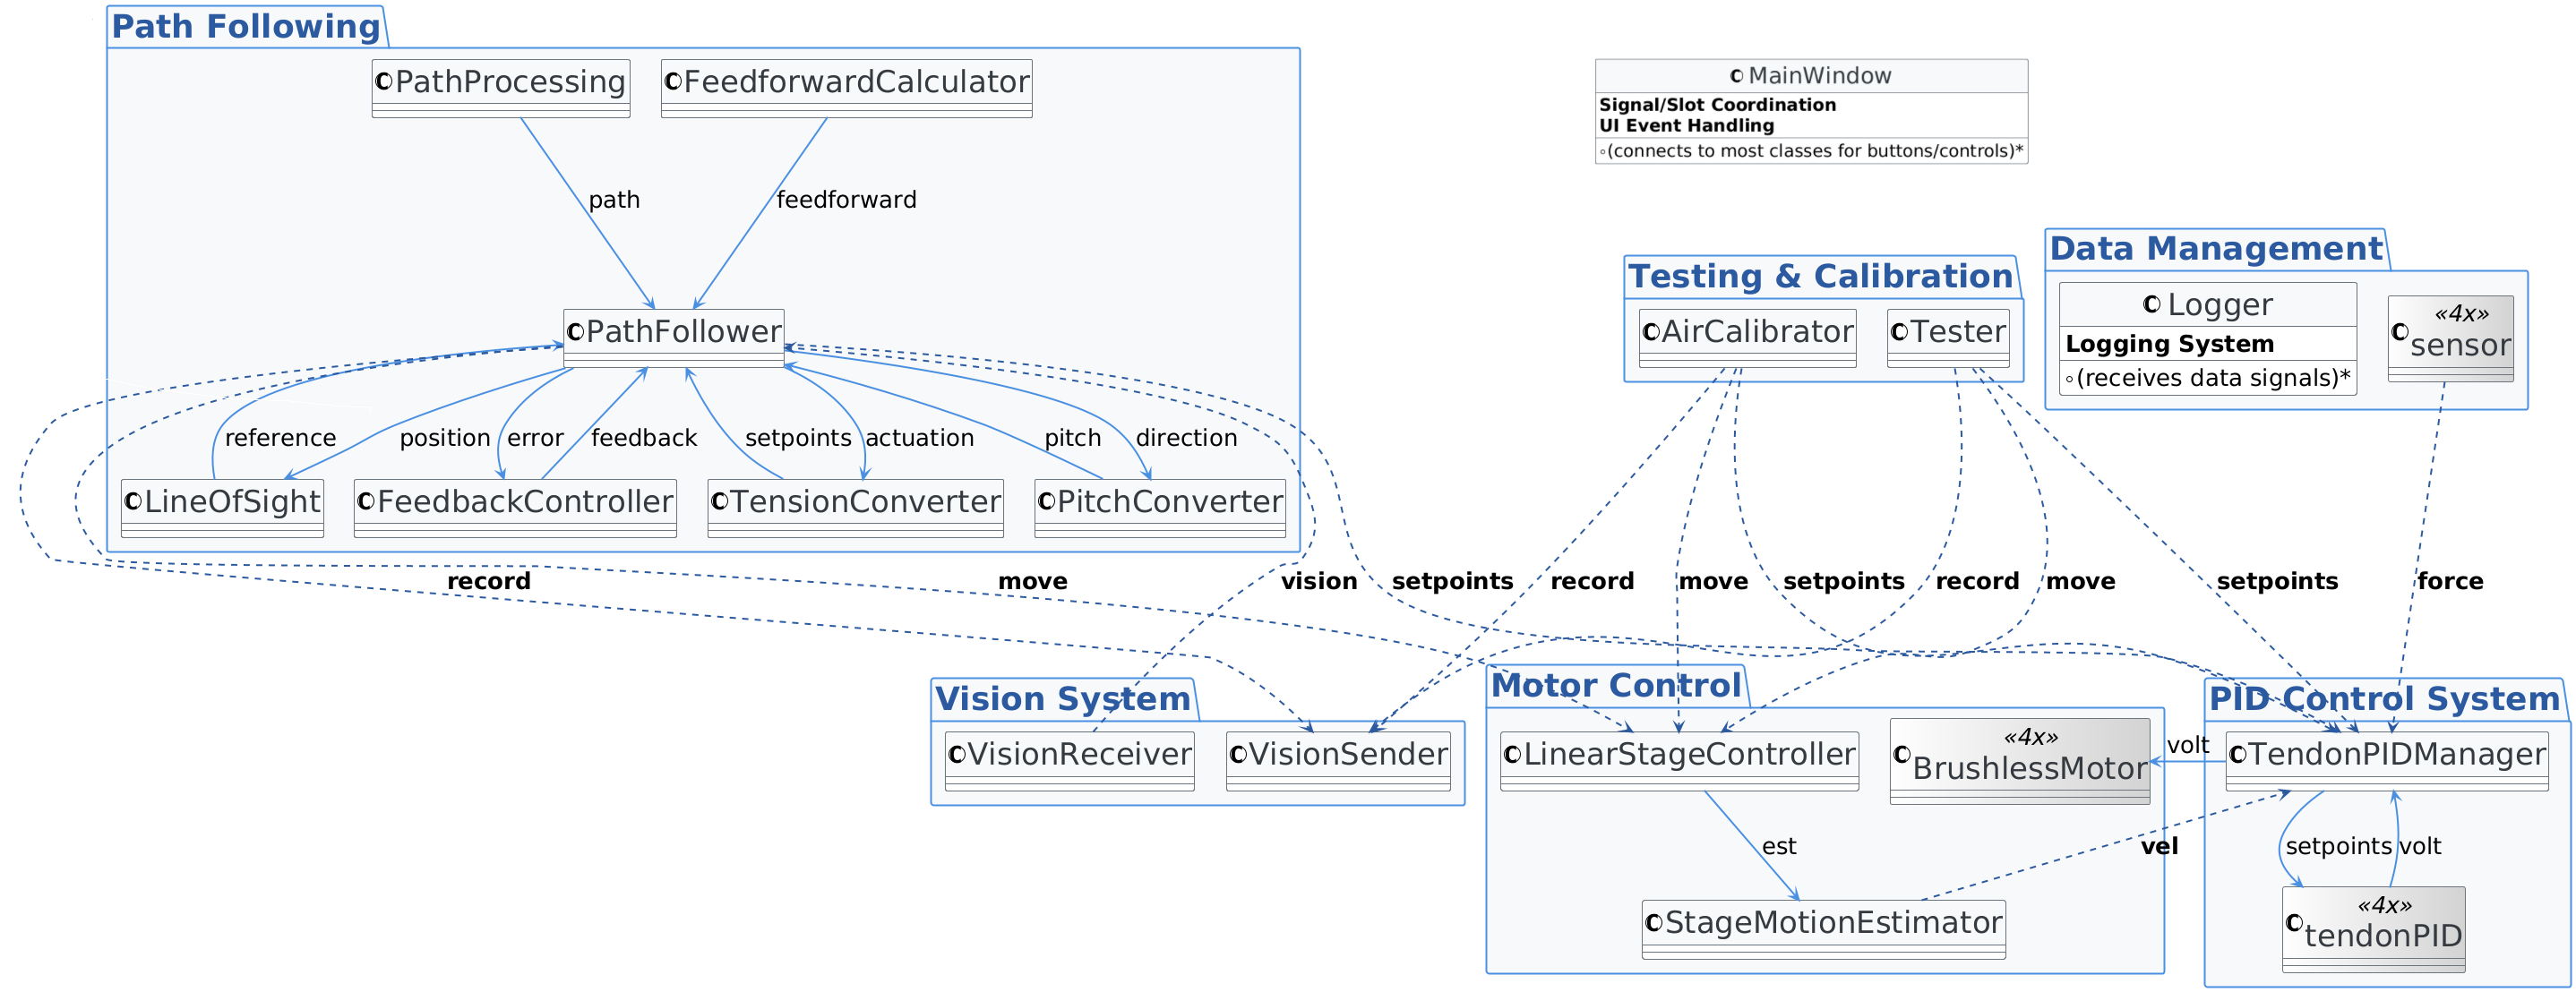
\includegraphics[width=1.1\linewidth]{images/Software documentation/architecture3.png}
	\caption{Final control code base architecture after refactoring}
	\label{fig:architecture}
\end{figure}
\leavevmode\newline
A visualization of the resulting architecture after refactoring can be seen in figure \ref{fig:architecture}. As shown, the system is now organized into modular, loosely coupled components with clear responsibilities. The architecture is also layered, with lower-level modules (such as hardware control and above that tendonpids) forming the foundation for higher-level logic (such as path following).






\subsubsection{Threading}
The entire system follows and event-driven architecture using Qt's signal-slot mechanisms wherever possible. This reduces the need for extensive multithreading as modules do not block threads for long periods. Instead most classes react to signals or timers. Some components, such as sensor data acquisition and closed-loop tension control, operate on fixed update intervals using timers. Others, like the path-following controller are triggered by receiving a new vision measurement.
\begin{figure} [H]
    \centering
    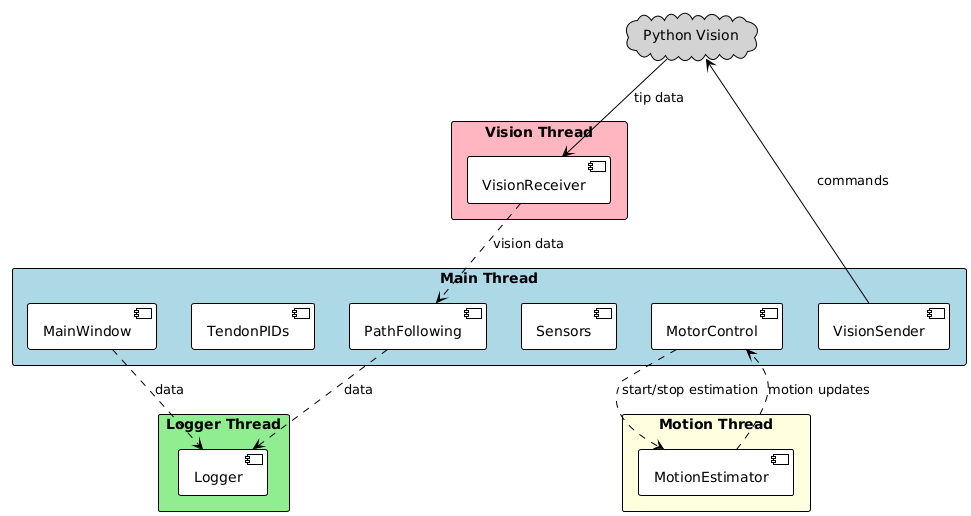
\includegraphics[width=0.95\linewidth]{images/Software documentation/threads.png}
    \caption{Visualization of communication between the 4 threads of the control system}
    \label{fig:threads}
\end{figure}
To support real-time performance and responsiveness, multithreading was introduced where strictly necessary. Only components that demonstrated clear performance bottlenecks or responsiveness issues were moved to separate threads. The components run in dedicated threads outside of the main thread are described in the following table. Additionally a figure \ref{fig:threads} visualizes the threads and the signals sent between them. 

\begin{table}[htbp]
\centering
\caption{Threading Architecture Description}
\begin{tabular}{p{0.3\textwidth}p{0.65\textwidth}}
\toprule
\textbf{Thread} & \textbf{Description} \\
\midrule
Logging Thread & Records sensor and control data without blocking the main loop. \\
\addlinespace
Motion Estimation Thread & Continuously estimates stage speed at a high frequency while the linear stage is running for use in feedforward for the closed loop tension control. \\
\addlinespace
Vision Receiver Thread & Continuously listens for incoming vision data and receives and parses it. \\
\bottomrule
\end{tabular}
\end{table}

\subsubsection{Graphical-User-Interface}
The graphical user interface (GUI) was completely redesigned to improve user-friendliness and expand the functionality of the system. Figure \ref{fig:oldgui} shows the old GUI before refactoring, while figure \ref{fig:gui} shows the new, refactored GUI.

\begin{figure}[H]
    \centering
    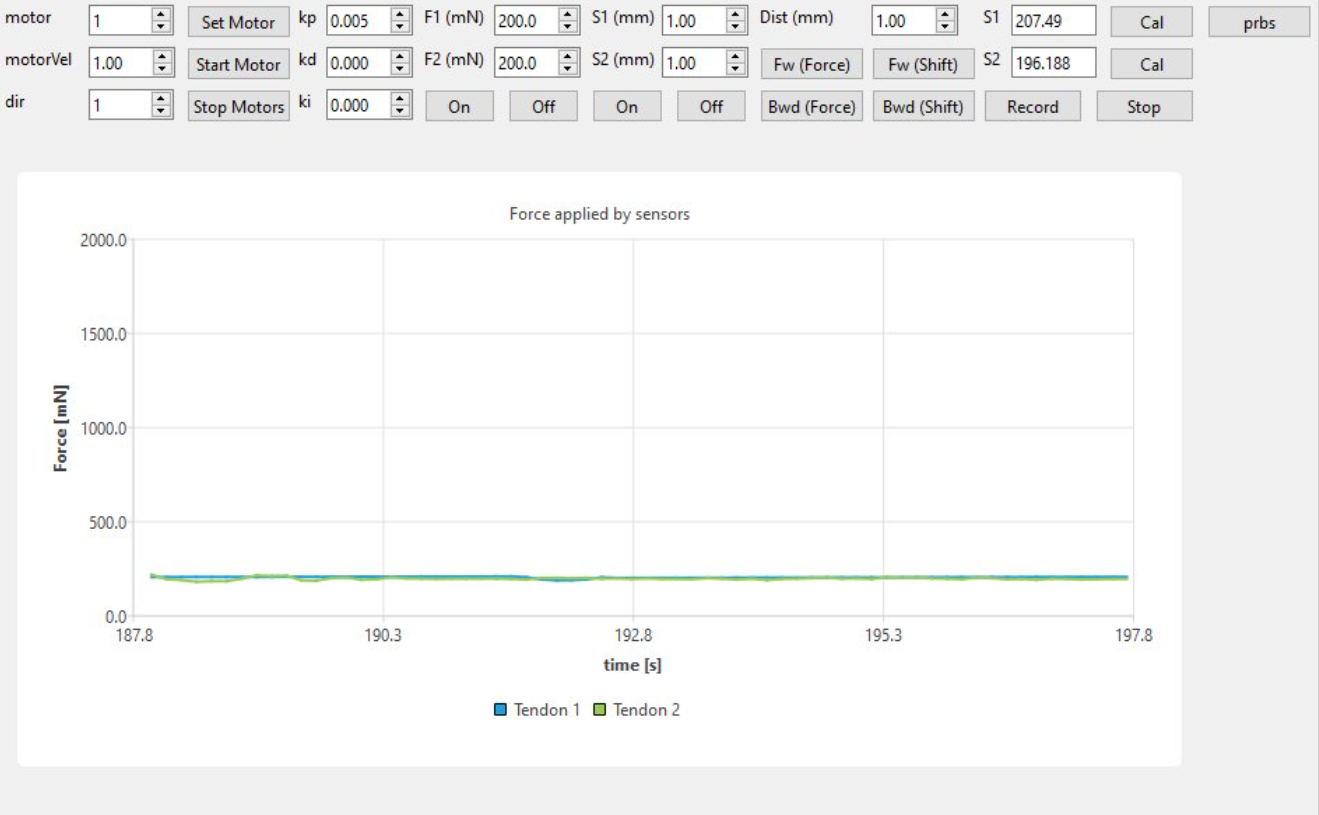
\includegraphics[width=0.95\linewidth]{images/gui/oldGUI.PNG}
    \caption{Old GUI before refactoring}
    \label{fig:oldgui}
\end{figure}
The original GUI had limited and sometimes unstable functionality with unclear labels. It was not entirely obvious what each button did, meaning that users were required to analyze the underlying code to use it effectively.

The redesigned GUI aims to have clearer organization with more functionality by grouping control according to their purpose. At the top left, the section labeled \texttt{Linear Stage} contains all controls relted to movement and speed settings for the linear actuator. To the right of this section are controls for logging and recording, which also include the ability to specify the desired target folder for the data.
\begin{figure} [H]
    \centering
    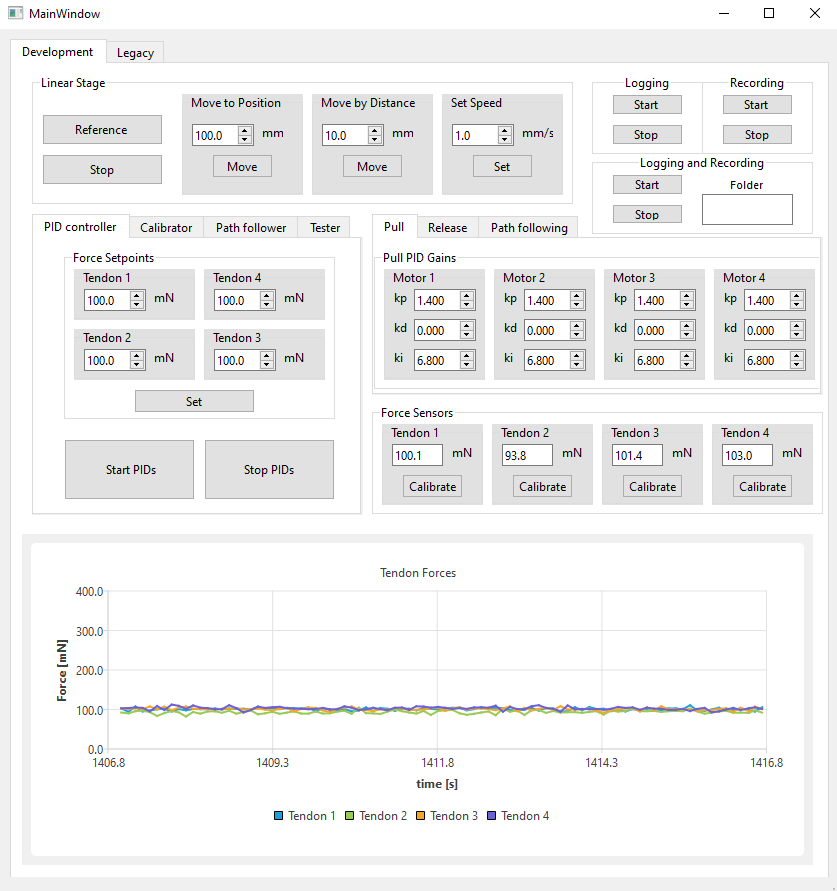
\includegraphics[width=0.85\linewidth]{images/gui/main.PNG}
    \caption{New GUI, after refactoring}
    \label{fig:gui}
\end{figure}
Below these sections to the left there are series of tabs that provide access to distinct operational modes, including PID control, air calibration, path following and testing routines. The tab section on the right-hand side relates to the setting of parameters. Users can use these tabs to configure the pull and release PID gains for each motor, as well as set parameters specific to the path-following algorithm.

The \texttt{Force Sensors} section presents a live view of the forces applied to each tendon, alongside a calibration button for each sensor. Finally at the bottom, a real-time plot visualizes the force data from all tendons and adjusts its y-axis scale to fit the range of values displayed.


\lhead{Software Refactoring - Discussion} % section header
\subsection{Discussion}
\subsubsection{Modularization}
While the original codebase was functional, it lacked the clarity and separation of concerns required for long-term maintainability and further development. The resulting system is both robust and significantly easier to work with. By redistributing the responsibilities from the \texttt{MainWindow} class to focused modules, the code base was made to better align with the principles of high cohesion and low coupling. The architectural redesign also established a clearer layering of the system, which allows each subsystem to evolve independently and simplifies debugging. The introduction of more clearly defined interfaces further improved the separation and readability.

\subsubsection{Threading}
The use of Qt's signal-slot, mechanism greatly reduced the risk of blocking operations and ensured responsiveness and the threading removes unnecessary delays in the control loop that could lead to instability. Importantly, threads were only added where clear performance issues were observed, rather than assigning a thread to every major module by default.

Some might argue that large modules that run their own closed loop control such as \texttt{PathFollowing} or \texttt{TendonPIDs} should also run in their own threads. While this could become relevant if the functionality expands significantly, current testing showed no significant lag or blocking from these modules since they operate at fixed timer-based intervals and do not require a lot of processing upon each call. It was therefore evaluated that adding additional threads would only introduce unnecessary complexity.

\lhead{Software Refactoring - Conclusion} % section header
\subsection{Conclusion}
Overall, the refactoring does more than clean up the code, it enables the development of new features, improves the reliability and readability and aligns the software with best practices for real-time, modular design. The resulting architecture is scalable, maintainable and better suited for future development

\lhead{Software Refactoring - Conclusion} % section header



